% BSD 3-Clause License
%
% Copyright (c) 2023, 2025 Quux System and Technology. All rights reserved.
%
% Redistribution and use in source and binary forms, with or without
% modification, are permitted provided that the following conditions are met:
%
% 1. Redistributions of source code must retain the above copyright notice, this
%    list of conditions and the following disclaimer.
%
% 2. Redistributions in binary form must reproduce the above copyright notice,
%    this list of conditions and the following disclaimer in the documentation
%    and/or other materials provided with the distribution.
%
% 3. Neither the name of the copyright holder nor the names of its
%    contributors may be used to endorse or promote products derived from
%    this software without specific prior written permission.
%
% THIS SOFTWARE IS PROVIDED BY THE COPYRIGHT HOLDERS AND CONTRIBUTORS "AS IS"
% AND ANY EXPRESS OR IMPLIED WARRANTIES, INCLUDING, BUT NOT LIMITED TO, THE
% IMPLIED WARRANTIES OF MERCHANTABILITY AND FITNESS FOR A PARTICULAR PURPOSE ARE
% DISCLAIMED. IN NO EVENT SHALL THE COPYRIGHT HOLDER OR CONTRIBUTORS BE LIABLE
% FOR ANY DIRECT, INDIRECT, INCIDENTAL, SPECIAL, EXEMPLARY, OR CONSEQUENTIAL
% DAMAGES (INCLUDING, BUT NOT LIMITED TO, PROCUREMENT OF SUBSTITUTE GOODS OR
% SERVICES; LOSS OF USE, DATA, OR PROFITS; OR BUSINESS INTERRUPTION) HOWEVER
% CAUSED AND ON ANY THEORY OF LIABILITY, WHETHER IN CONTRACT, STRICT LIABILITY,
% OR TORT (INCLUDING NEGLIGENCE OR OTHERWISE) ARISING IN ANY WAY OUT OF THE USE
% OF THIS SOFTWARE, EVEN IF ADVISED OF THE POSSIBILITY OF SUCH DAMAGE.
%
\RequirePackage[l2tabu, orthodox]{nag}
\documentclass{cookbook}
\input{git-revision.tex}
\usepackage{bookmark}
\usepackage{hyperxmp}
\usepackage{totpages}
\AtBeginDocument{%
	\hypersetup{%
		pdfpagerange={1-\ref*{TotPages}},
		pdfnumpages={\ref*{TotPages}}
	}%
}
	\hypersetup{
		unicode=true,
		pdfduplex={DuplexFlipLongEdge},
		pdfprintscaling={AppDefault},
		pdfpicktraybypdfsize={true},
		pdfcreator={XeLaTeX},
		pdfproducer={Quux Script-Shift Scribe},
		pdftoolbar={true},
		pdftitle={Sichuan Cookbook 1972 Remake (Preview)},
		pdfsubject={312 Traditional Recipes: The Culinary History of Sichuan},
		pdfauthor={Chengdu Catering Company},
		pdfauthortitle={},
		pdfcopyright={Copyright (c) 2023--2025 Quux System and Technology},
		pdfkeywords={Chinese-food, cookbook, culture, food, recipe, %
			Sichuan, Szechuan, Szechwan},
		pdflicenseurl={https://opensource.org/license/bsd-3-clause},
		pdfcaptionwriter={GONG Jie},
		pdfcontactaddress={},
		pdfcontactcity={Fengtai District},
		pdfcontactregion={Beijing Municipality},
		pdfcontactcountry={China},
		pdfcontactpostcode={100000},
		pdfcontactemail={},
		pdfcontactphone={},
		pdfcontacturl={%
			https://leanpub.com/sichuan-cookbook/
		},
		pdfdocumentid={uuid:4da76418-2c77-4d51-be82-c4926dd533a3},
		pdfversionid={v1.0.6},
		pdfpublication={},
		pdfpublisher={Quux System and Technology},
		pdfpubtype={book},
		pdfvolumenum={0},
		pdfissuenum={0},
		pdfisbn={0},
		pdfbookedition={[en]First electronic edition},
		pdflang={zh-CN},
		pdfmetalang={en},
		pdfurl={https://leanpub.com/s/B0263A83D1DB443FA1FF336F9EA4E822.pdf},
		pdfdoi={},
		pdfidentifier={},
		pdfbytes={3653600},
		pdfinfo={
			GitCommitName={\gitcommitname},
			GitCommitHash={\gitcommithash},
			GitCommitterDate={\gitcommitterdate},
			PDFBuildDate={\pdfbuilddate},
			PDFBuildHost={\pdfbuildhost}
		},
		hidelinks
	}
	\XMPLangAlt{zh-TW}{
		pdftitle={四川食譜1972重製版（預覽版）},
		pdfsubject={312道傳統食譜：四川美食的歷史},
		pdfcopyright={版權所有 (c) 2023--2025 餛飩系統與科技}
	}
	\XMPLangAlt{zh-CN}{
		pdftitle={四川菜谱1972重制版（预览版）},
		pdfsubject={312道传统菜谱：四川美食的历史},
		pdfcopyright={版权所有 (c) 2023--2025 馄饨系统与科技}
	}
	\XMPLangAlt{fr}{
		pdftitle={Recette du Sichuan 1972 Remake (Aperçu)},
		pdfsubject={312 Recettes Traditionnelles : L'Histoire Culinaire du Sichuan},
		pdfcopyright={Copyright (c) 2023--2025 Quux System and Technology}
	}
	\XMPLangAlt{de}{
		pdftitle={Sichuan Kochbuch 1972 Remake (Vorschau)},
		pdfsubject={312 traditionelle Rezepte: Die kulinarische Geschichte von Sichuan},
		pdfcopyright={Urheberrecht (c) 2023–-2025, Quux System und Technologie}
	}
	\XMPLangAlt{es}{
		pdftitle={Recetario de Sichuan 1972 Remake (Avance)},
		pdfsubject={312 Recetas Tradicionales: La Historia Culinaria de Sichuan},
		pdfcopyright={Derechos de autor (c) 2023–2025, Quux System and Technology}
	}
	\XMPLangAlt{ru}{
		pdftitle={Кулинарная книга Сычуани 1972 Ремейк (Предварительный Просмотр)},
		pdfsubject={312 традиционных рецептов: Кулинарная история Сычуани},
		pdfcopyright={Авторское право (c) 2023--2025 Quux System and Technology}
	}
	\XMPLangAlt{ja}{
		pdftitle={四川料理本1972リメイク版（プレビュー）},
		pdfsubject={312の伝統的なレシピ：四川料理の歴史},
		pdfcopyright={著作権 (c) 2023--2025 ククスシステムとテクノロジー}
	}
	\XMPLangAlt{kr}{
		pdftitle={사천 요리책 1972 리메이크（시사）},
		pdfsubject={312개의 전통 요리법：쓰촨 요리의 역사},
		pdfcopyright={저작권 (c) 2023--2025 퀙스 시스템과 기술}
	}
\usepackage{pdfpages}
\usepackage{pdfoverlay}

\newcommand{\blankpage}[1]{%
	\thispagestyle{empty}
	\begingroup%
	\null%
	\vfill%
	\begin{center}
	\zihao{3}\kafamily%
	第#1页不包括\\ 在此预览版之内。
	\end{center}
	\vfill%
	\endgroup%
	\clearpage
	\thispagestyle{empty}
	\begingroup%
	\null%
	\vfill%
	\begin{center}
	\zihao{3}\kafamily%
	此页故意留白。
	\end{center}
	\vfill%
	\endgroup%
}%

\begin{document}
\begin{cookbook}

\pagestyle{empty}
\pagenumbering{Alph}%	Upper case letter page numbers (and reset to 1)
\bookmarksetup{startatroot}%
% Front cover
\hypertarget{front-cover}{}%
\bookmark[dest=front-cover,level=section]{封面}%
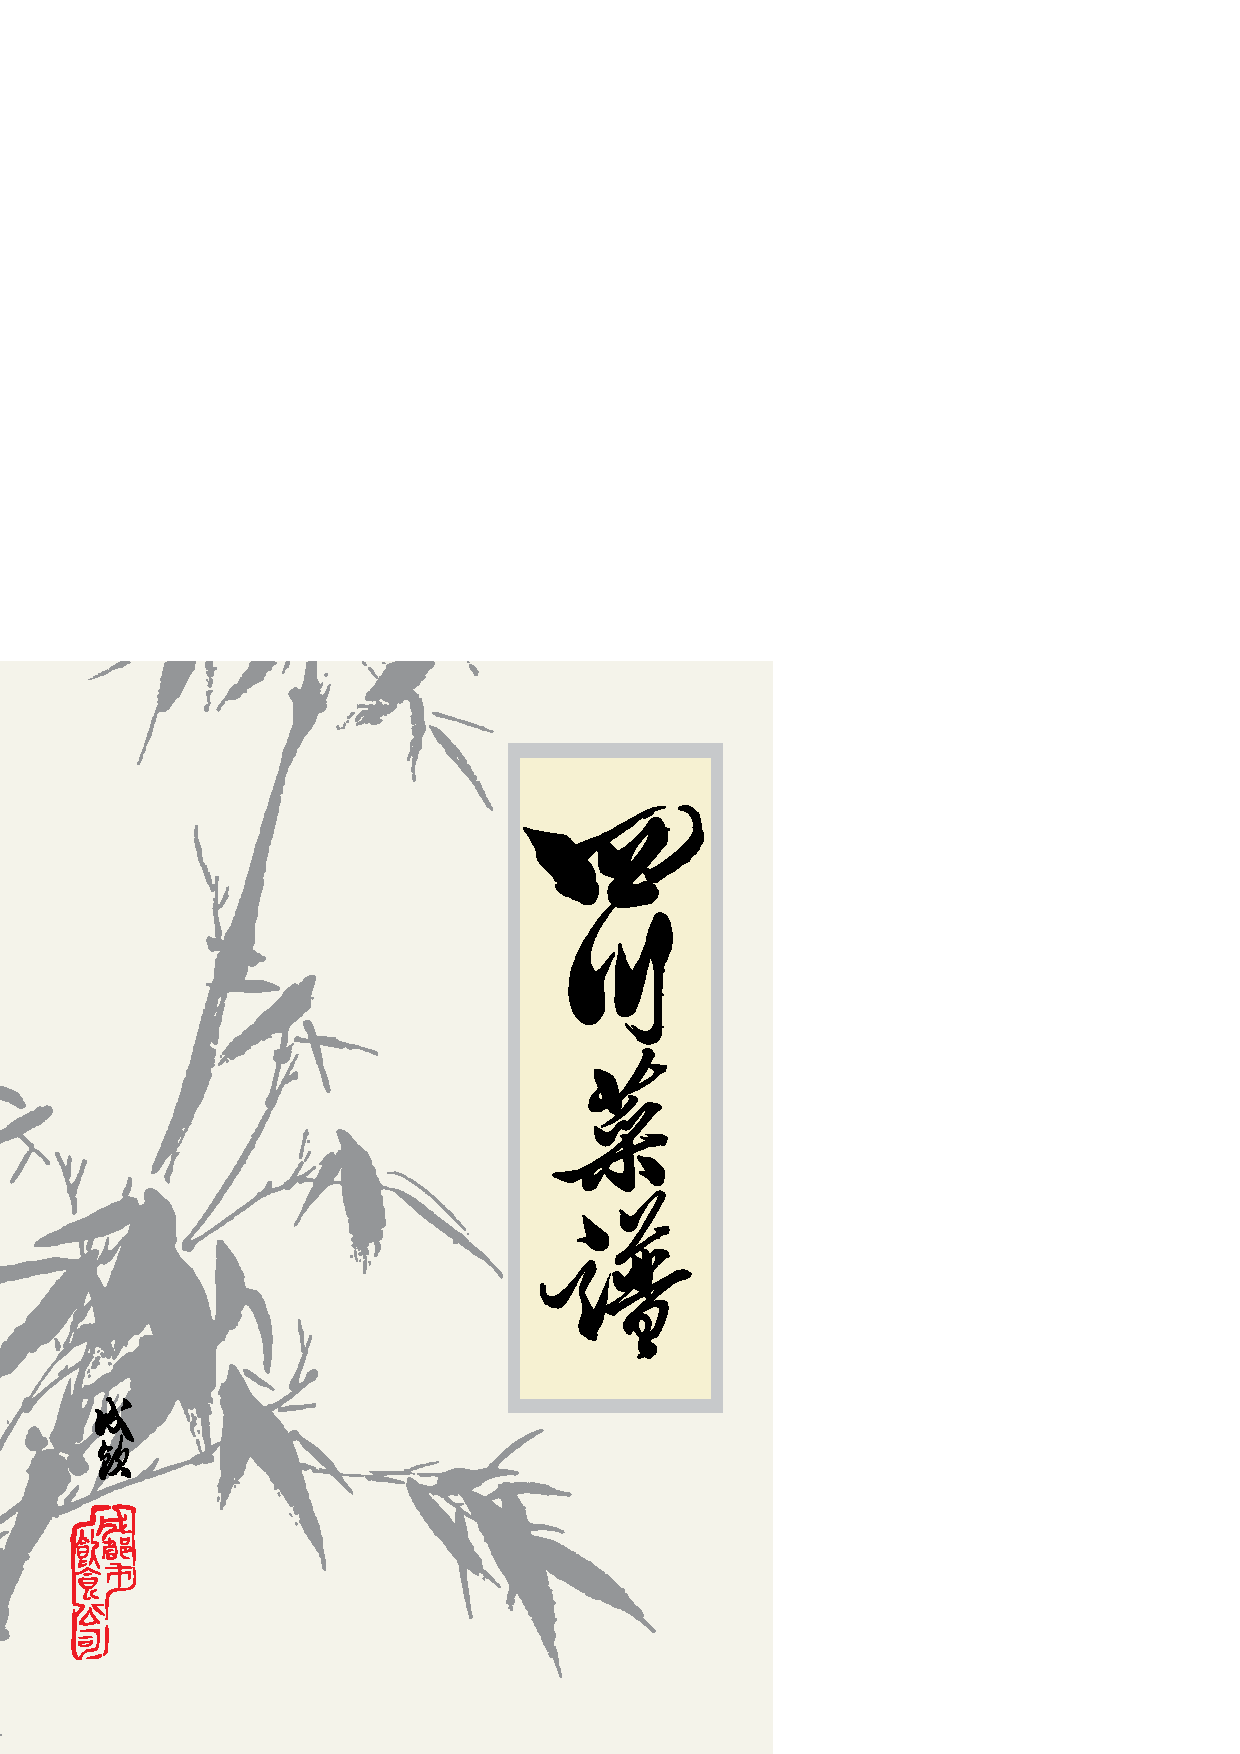
\includepdf[pages=1]{sichuan-cookbook.pdf}
\clearpage
\hypertarget{inside-front-cover}{}%
\bookmark[dest=inside-front-cover,level=section]{封二}%
\includepdf[pages=2]{sichuan-cookbook.pdf}
\cleardoublepage

\hypertarget{half-title}{}%
\bookmark[dest=half-title-page,level=section]{书名页}%
\pdfoverlaySetPDF{preview.pdf}
\includepdf[pages=3]{sichuan-cookbook.pdf}
\cleardoublepage

\hypertarget{frontispiece}{}%
\bookmark[dest=frontispiece,level=section]{卷首插图}%
\pdfoverlaySetPDF{preview.pdf}
\includepdf[pages=5]{sichuan-cookbook.pdf}
\cleardoublepage

\hypertarget{title-page}{}%
\bookmark[dest=title-page,level=section]{标题页}%
\pdfoverlaySetPDF{preview.pdf}
\includepdf[pages=7]{sichuan-cookbook.pdf}
\clearpage
\hypertarget{copyright-page}{}%
\bookmark[dest=copyright-page,level=section]{版权页}%
\pdfoverlaySetPDF{sample.pdf}
\includepdf[pages=8]{sichuan-cookbook.pdf}
\cleardoublepage

\hypertarget{quotes-from-chairman-mao}{}%
\bookmark[dest=quotes-from-chairman-mao,level=section]{毛主席语录}%
\includepdf[pages=9]{sichuan-cookbook.pdf}
\cleardoublepage

% Title page 1972
\hypertarget{title-page-1972}{}%
\bookmark[dest=title-page-1972,level=section]{1972年标题页}%
\includepdf[pages=11]{sichuan-cookbook.pdf}
\cleardoublepage

% Editorial notes 1972
\hypertarget{editorial-notes-1972}{}%
\bookmark[dest=editorial-notes-1972,level=section]{1972年编印说明}%
\includepdf[pages=13]{sichuan-cookbook.pdf}
\cleardoublepage

\frontmatter

\pagestyle{fancy}
\hypertarget{table-of-contents}{}%
\bookmark[dest=table-of-contents,level=section]{目录}%
\includepdf[pages={15-21}]{sichuan-cookbook.pdf}

\mainmatter

\hypertarget{chapter1}{}%
\bookmark[dest=chapter1,level=chapter]{肉食类}%
\includepdf[pages={23-26}]{sichuan-cookbook.pdf}
\cleardoublepage

\hypertarget{chapter2}{}%
\bookmark[dest=chapter2,level=chapter]{鸡鸭类}%
\hypertarget{chapter3}{}%
\bookmark[dest=chapter3,level=chapter]{鱼虾类}%
\blankpage{5--194}
\cleardoublepage

\setcounter{page}{195}%
\hypertarget{chapter4}{}%
\bookmark[dest=chapter4,level=chapter]{山海味类}%
\includepdf[pages={217-218}]{sichuan-cookbook.pdf}
\cleardoublepage

\hypertarget{chapter5}{}%
\bookmark[dest=chapter5,level=chapter]{甜食类}%
\hypertarget{chapter6}{}%
\bookmark[dest=chapter6,level=chapter]{蔬菜类}%
\hypertarget{chapter7}{}%
\bookmark[dest=chapter7,level=chapter]{其它类}%
\hypertarget{chapter8}{}%
\bookmark[dest=chapter8,level=chapter]{重庆市部分菜肴}%
\blankpage{197--300}
\cleardoublepage

\appendix

\setcounter{page}{301}%
\bookmarksetup{startatroot}%
\hypertarget{collation-notes}{}%
\bookmark[dest=collation-notes,level=section]{校勘记}%
\includepdf[pages={323-324}]{sichuan-cookbook.pdf}
\cleardoublepage
\blankpage{303--308}
\cleardoublepage
\hypertarget{index}{}%
\bookmark[dest=index,level=section]{索引}%
\includepdf[pages={331-332}]{sichuan-cookbook.pdf}
\cleardoublepage
\blankpage{311--326}
\cleardoublepage

\backmatter

\pagestyle{empty}
\pagenumbering{Alph}%   Upper case letter page numbers (and reset to 1)
\setcounter{page}{25}%  Letter Y
\bookmarksetup{startatroot}%
\hypertarget{inside-back-cover}{}%
\bookmark[dest=inside-back-cover,level=section]{封三}%
\includepdf[pages={351}]{sichuan-cookbook.pdf}
\clearpage

% Back cover
\hypertarget{back-cover}{}%
\bookmark[dest=back-cover,level=section]{封底}%
\includepdf[pages={352}]{sichuan-cookbook.pdf}

\end{cookbook}
\end{document}

% vim: filetype=tex noautoindent nojoinspaces
% vim: fileencoding=utf-8 formatoptions+=m
% vim: textwidth=78 tabstop=4 shiftwidth=4 softtabstop=4
